\documentclass[a4paper,12pt,oneside]{book}
\usepackage[export]{adjustbox}
\usepackage{graphicx}
\usepackage[margin=2cm]{geometry}
\usepackage{color}
\usepackage{fix-cm}  
\usepackage{fancyhdr}  


\usepackage[scale=2,opacity=0.1,angle=0]{background}
\backgroundsetup{contents={
\includegraphics{logo}}}

\definecolor{Dred}{RGB}{210,0,0}
\definecolor{Dblue}{RGB}{0,0,150}


\begin{document}
%\maketitle
%\tableofcontents
\begin{titlepage}
\hspace{5cm}
\textit{\textcolor{Dblue}{\textbf{\fontsize{60}{70}\selectfont{Fi-Pi}}}}
\\\\\\\\\\
\textcolor{Dred}{\textbf{\fontsize{30}{10}\selectfont{Adaptor Board for Firebird V Robot}}}
\\\\\
\textcolor{Dred}{\textbf{\fontsize{30}{10}\selectfont{\hspace{4 cm}using Raspberry Pi 2}}}
\\\\\\\\
\textcolor{Dred}{\textbf{\fontsize{30}{10}\selectfont{\hspace{3 cm}HARDWARE MANUAL}}}
\\\\\\\\

\begin{figure}[h]
		\hspace{3cm}
	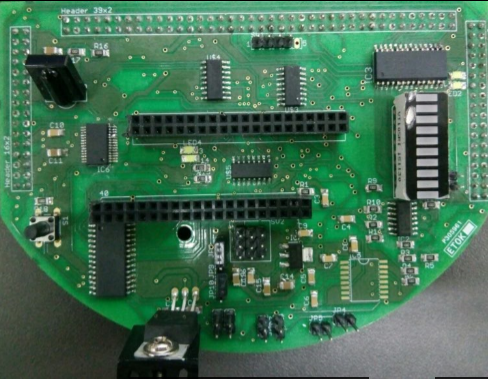
\includegraphics[width=0.8\textwidth]{pcb}
\end{figure}
\hfill
\end{titlepage}
\pagebreak

\pagestyle{fancy}
\fancyhf{}
\rhead{Fi-Pi hardware manual}
\lfoot{www.eyantra.org}
\rfoot{Page \thepage}
.\\
\textbf{\fontsize{10}{10}\selectfont{Documentation author}}
\\\\
\hspace{5cm}
Milan Preet Singh
\\\
Tejaswini A
\\\\
\textbf{\fontsize{10}{10}\selectfont{Mentors}}
\\\\
\hspace{5cm}
Rutuja
\\\
Deepa
\pagebreak

\pagestyle{fancy}
\fancyhf{}
\rhead{Fi-Pi hardware manual}
\lfoot{www.eyantra.org}
\rfoot{Page \thepage}
\textbf{\fontsize{30}{10}\selectfont{\hspace{5 cm}INDEX}}\\\\
\begin{enumerate}
	\item {\fontsize{15}{10}\selectfont{Introduction}}
    \item {\fontsize{15}{10}\selectfont{Main board pin details}}
	\item {\fontsize{15}{10}\selectfont{Powering Raspberry Pi}}
	\item {\fontsize{15}{10}\selectfont{Battery voltage indication}}
	\item {\fontsize{15}{10}\selectfont{Buzzer interface}}
    \item {\fontsize{15}{10}\selectfont{LCD interface}}
    \item {\fontsize{15}{10}\selectfont{Sensors and ADC interface}}
    \item {\fontsize{15}{10}\selectfont{Motors and wheel encoders interface}}
    \item {\fontsize{15}{10}\selectfont{Powering servo motors and Servo pod connections}}
    \item {\fontsize{15}{10}\selectfont{Interrupt switch and controlling bargraph leds}}
    \item {\fontsize{15}{10}\selectfont{TSOP1738 RC5 IR receiver and decoder}}
    \item {\fontsize{15}{10}\selectfont{Xbee communication}}
    \item {\fontsize{15}{10}\selectfont {FT232 USB to serial converter}}
    \item {\fontsize{15}{10}\selectfont{TTL to RS232 converter}}
    \item {\fontsize{15}{10}\selectfont{UART communication with Raspberry Pi}}
    \item {\fontsize{15}{10}\selectfont{Adaptor board expansion socket}} 
\end{enumerate}
\pagebreak

\section*{\textbf{\fontsize{25}{10}\selectfont{1.Introduction}}}

Currently Firebird V robot comes with ATMEGA2560, 8051, ARM7 adaptor board. Using a raspberry pi based adaptor board would add to the functionality of the robot. The idea is to integrate the features of RPi to Firebird V robot.This would facilitate any on-board computations, image processing(Rpi supports PiCamera directly), the robot could even be used for IOT applications. Because of the presence of an operating system, Rpi is a mini computer.Adaptor board for Firebird V would definitely be an advantage.\\
\hfill

\subsection*{\textbf{Components on the adaptor board}}
\vspace{1cm}
\begin{itemize}
	\item{MCP3008 (8 channel 10-bit ADC)}
	\item{MCP23017 Port expander IC}
	\item{Header pins for interfacing adaptor board with main board, raspberry pi and for the expansion socket.}
	\item{FT232 for USB communication}	
	\item{MAX202 for RS232 communication}
	\item{LM324 quad comparator IC}
	\item{Bar Graph LED}
	\item{L7805 IC for powering Rpi}
	\item{LM1117 IC for powering servo motors}
	\item{Switches}
    \item{Jumpers}
    \item{Resistors,capacitors,diodes,LEDs}	
\end{itemize}
\pagebreak

\section*{\textbf{\fontsize{25}{10}\selectfont{2.Main board pin details}}}
\begin{figure}[h]
	%	\hspace{5cm}
	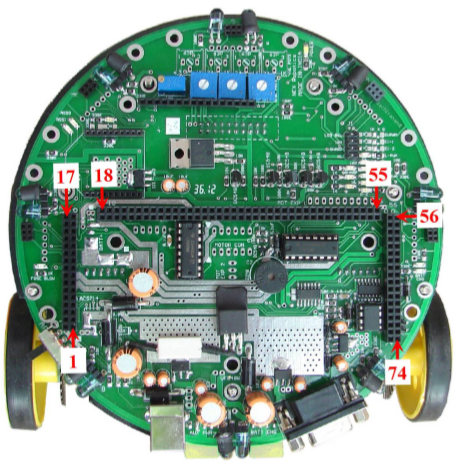
\includegraphics[width=1.\textwidth]{main_board}
\end{figure}

\begin{tabular}{|p{2cm}|p{4cm}|p{10cm}|}
	\hline
\textbf{Pin No.} & \textbf{Pin Name} & \textbf{Function}\\ [0.5ex] 
\hline
1. & CS\* &Current sense analog value  \\ 
\hline
2. & IR Proximity sensor 8 &IR Proximity sensor 8 analog value  \\ 
\hline
3. &Ground &Ground  \\ 
\hline
4. &USB Data+ &USB connection going to the raspberry pi via FT232 USB to serial converter.To enable USB communication set jumper as shown.  \\ 
\hline
5. &USB Data- &USB connection going to the raspberry pi via FT232 USB to serial converter.To enable USB communication set jumper as shown. \\ 
\hline
6. &VUSB &Voltage source for FT232  \\ 
\hline

\end{tabular}
\pagebreak 

\begin{tabular}{|p{2cm}|p{4cm}|p{10cm}|}

	\hline
	7. &5V System &5V System Voltage. Can be used for powering up any digital device with current limit of 400mA  \\ 
	\hline
8. &5V Sensor &5V Sensor Voltage. Can be used for additional sensor interfacing with current limit 300mA. \\ 
\hline
9. &5V Sensor &5V Sensor Voltage. Can be used for additional sensor interfacing with current limit 300mA. \\ 
\hline
	10. &5V System &5V System Voltage. Can be used for powering up any digital device with current limit of 400mA  \\ 
\hline
	11. &Sharp IR Range Sensor 1 &Analog output of Sharp IR range Sensor 1 \\ 
	\hline
12. &IR Proximity Sensor 1 &Analog output of IR Proximity Sensor 1. \\ 
\hline
	13. &XBee RXD & XBee wireless module serial data in  \\ 
	\hline
14. &XBee TXD & XBee wireless module serial data out  \\ 
\hline
15. &Sharp IR Range Sensor 2 &Analog output of Sharp IR range Sensor 2 \\ 
\hline
16. &IR Proximity Sensor 2 &Analog output of IR Proximity Sensor 2. \\ 
\hline
17A. &RSSI &To capture the RSSI signal \\
\hline
17B.& Ultrasonic Trigger& To give trigger for Ultrasonic sensor \\
\hline
18.& MOSI & SPI Communication line for communicating with raspberry pi. Master Out Slave In. \\
\hline
19.& MISO & SPI Communication line for communicating with raspberry pi. Master In Slave Out. \\
\hline
20.& SCK & SPI Communication line for communicating with raspberry pi. Clock signal. \\
\hline 
21.& SSI & SPI Communication line for communicating with raspberry pi. \\
\hline
22. & RS & LCD Register select pin(Command)\\
\hline
23. & RW & LCD Write pin(Command)\\
\hline
24. & EN & LCD Enable pin(Command)\\
\hline
25. & DB5 & LCD Data bit 5\\
\hline
26. & DB4 & LCD Data bit 4\\
\hline
27. & DB5 & LCD Data bit 6\\
\hline
28. & DB5 & LCD Data bit 7\\
\hline
29. & V Battery System & 9-12V unregulated power supply for additional module interfacing.\\
\hline
30. & White Line sensor 1 & Analog output of White Line sensor 1\\
\hline
31. & White Line sensor 2 & Analog output of White Line sensor 2\\
\hline
32. & White Line sensor 3 & Analog output of White Line sensor 3\\
\hline
33. & Sharp IR Sensor 1 to 5 Disable &TTL or CMOS input.Disable IR range Sensor\\
\hline
34. &IR Proximity Sensor Disable &TTL or CMOS input.Disable IR range Sensor\\
	\hline
35. &5V System &5V System Voltage. Can be used for powering up any digital device with current limit of 400mA  \\ 
\hline
36. & White Line sensor 4 & Analog output of White Line sensor 4\\
\hline
37. & White Line sensor 5 & Analog output of White Line sensor 5\\
\hline
38. & White Line sensor 6 & Analog output of White Line sensor 6\\
\hline
39. & White Line sensor 7 & Analog output of White Line sensor 7\\
\hline
\end{tabular}
\pagebreak 

\begin{tabular}{|p{2cm}|p{4cm}|p{10cm}|}
	\hline
40. & White Line Sensor Disable &TTL or CMOS input.Disable White Line Sensor\\
\hline
41. &Sharp IR Range Sensor 3 &Analog output of Sharp IR range Sensor 3 \\ 
\hline
42. &IR Proximity Sensor 3 &Analog output of IR Proximity Sensor 3. \\ 
\hline
43. &IR Proximity Sensor 4 &Analog output of IR Proximity Sensor 4. \\
\hline 
44. &Sharp IR Range Sensor 4 &Analog output of Sharp IR range Sensor 4 \\
\hline 
45. &Sharp IR Range Sensor 5 &Analog output of Sharp IR range Sensor 5 \\ 
\hline
46. &IR Proximity Sensor 5 &Analog output of IR Proximity Sensor 5. \\
\hline
47. & C1 1 & Logic input 1 for C1 Motor Drive\\
\hline
48. & C1 PWM & PWM input for C1 Motor Drive\\
\hline
49. & C1 2 & Logic input 2 for C1 Motor Drive\\
\hline
50. & PWML & PWM input for Left Motor Drive\\
\hline
51. & L1 & Logic input 1 for Left Motor Drive\\
\hline
52. & L2 & Logic input 2 for Left Motor Drive\\
\hline
53. & R1 & Logic input 1 for Right Motor Drive\\
\hline
54. & PWMR & PWM input for Right Motor Drive\\
\hline
55. & R2 & Logic input 2 for Right Motor Drive\\
\hline
56. & & Not Used\\
\hline
57. & & Not Used\\
\hline
58. & & Not Used\\
\hline
59. & & Not Used\\
\hline
60. & & Not Used\\
\hline
61. & & Not Used\\
\hline
62. &Position Encoder Left &Output of Left Position Encoder (0-5V)\\
\hline
63. &Position Encoder Right &Output of Right Position Encoder (0-5V)\\
\hline
64. &Position Encoder C2 &Output of C2 Position Encoder (0-5V)\\
\hline
65. &Position Encoder C1 &Output of C1 Position Encoder (0-5V)\\
\hline
66. & C2 2 & Logic input 2 for C2 Motor Drive\\
\hline
67. & C2 1 & Logic input 1 for C2 Motor Drive\\
\hline
68. & C2 PWM & PWM input for C2 Motor Drive\\
\hline
69. &IR Proximity Sensor 6 &Analog output of IR Proximity Sensor 6. \\
\hline
70. &IR Proximity Sensor 7 &Analog output of IR Proximity Sensor 7. \\
\hline
71. &Buzzer &Input, V>0.65V turns on the buzzer \\
\hline
72. &DAC OUT &Not Connected \\
\hline
73. &RS232 TXD & RS232 Transmit, connected to DB9 serial connector on main board \\
\hline
74. &RS232 RXD & RS232 Receive, connected to DB9 serial connector on main board \\
\hline


 
\end{tabular}
\pagebreak 

\section*{\textbf{\fontsize{25}{10}\selectfont{3.Powering Raspberry Pi}}}
\begin{figure}[h]
%	\hspace{5cm}
	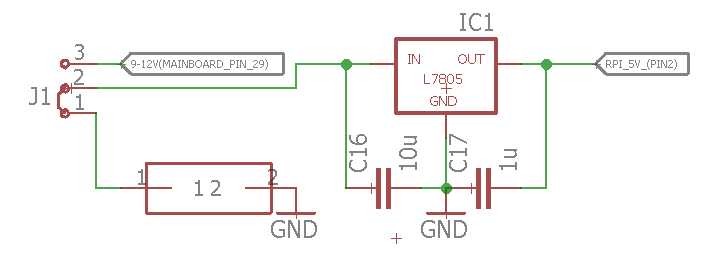
\includegraphics[width=1.\textwidth]{rpi_power}
\end{figure}
\hfill
\begin{itemize}
	\item{Raspberry pi needs a constant 5v and more than 1A power supply. L7805 voltage regulator is used to serve this purpose.}
	\item {The battery voltage of Firebird V robot is directly obtained by using pin 29 of main board.}
	\item {The output of 29th pin on the main board is in the range of 9-12v. Either this or any external battery can be used as an input for the 7805 IC. The selection between the two is facilitated by a jumper.}
	\item {The output of 7805 is the regulated 5v output, which is given to 5v pin of raspberry pi.}
	\item {Two header pins are provided for the connection with external battery.}
\end{itemize}
\pagebreak

\section*{\textbf{\fontsize{25}{10}\selectfont{4.Battery voltage indication}}}

\begin{figure}[h]
	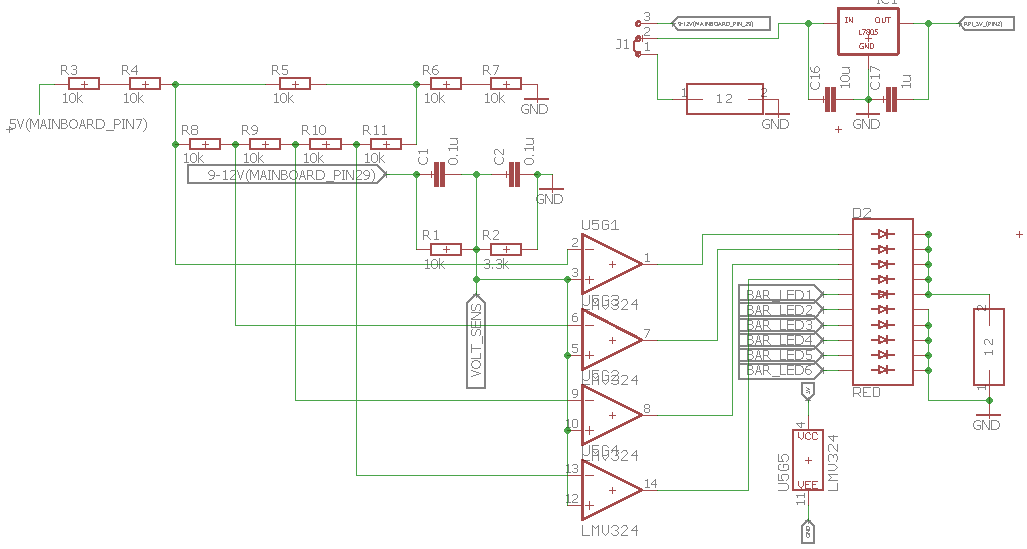
\includegraphics[width=1\textwidth]{volt_sens}
\end{figure}
\hfill
\begin{itemize}
	\item{The battery voltage of the Firebird V robot can be detected by the battery voltage sensing circuit.}
	\item{It could be sensed either by connecting the volt\_sens pin to ADC and reading its value or by seeing the indications from the bottom 5 LEDs of bargraph LEDs}
	\item{First of all, the 9-12v output from mainboard pin 29 is mapped to value less than 5V by using the voltage divider circuit.This circuit apprx divides the voltage by 4 and henceforth mapping 12V to 3V, 11V to 2.75V, 10V to 2.5V and 9V to 2.25V.This output is given to all 4 input+ pins of the quad comparator IC LM324.}
	\item{The input for input- pins are given as 3V, 2.75V, 2.5V, 2.25V resp by the simple circuit as given above.}
%	\item{The four outputs of LM324 is given to lower \+ve pins of bargraph LED (Last 2 pins shorted).}
	\item{So, whenever voltage is greater than 12V all the bottom 5 LEDs glow, when greater than 11V and less than 12V bottom 4 LEDs glow, when greater than 10V and less than 11V bottom 3 LEDs glow and when greater than 9V and less than 10V bottom 2 LEDs glow.}
	\item {In order to see the battery status, jumper has to be inserted into the two header pins provided at te right of the bargraph LED.}
\end{itemize}
\pagebreak

\section*{\textbf{\fontsize{25}{10}\selectfont{5.Buzzer interface}}}
\begin{figure}[h]
	
	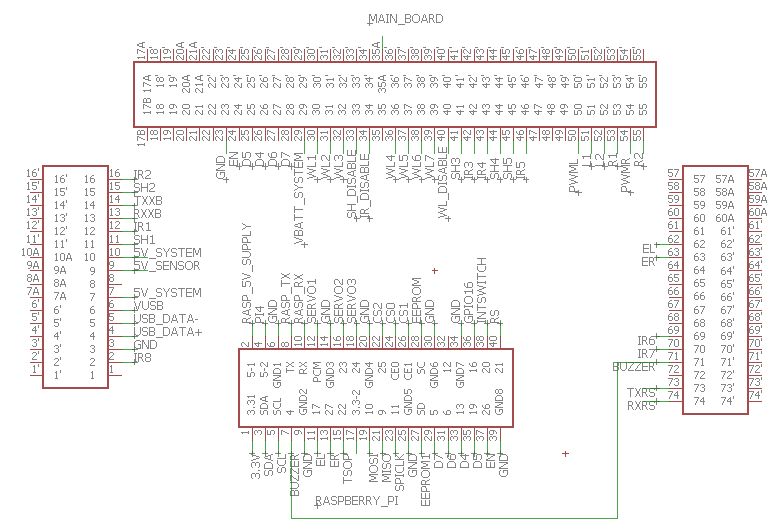
\includegraphics[width=1\textwidth]{buzzer}
\end{figure}
\hfill
\begin{itemize}
	\item {Input for buzzer is available at pin 71 of main board.}
	\item {This input is given to GPA6 of port expander 1.}
	\item {In order to program it, this pin should be used.}
\end{itemize}
\pagebreak

\section*{\textbf{\fontsize{25}{10}\selectfont{6.LCD interface}}}
\begin{figure}[h]
	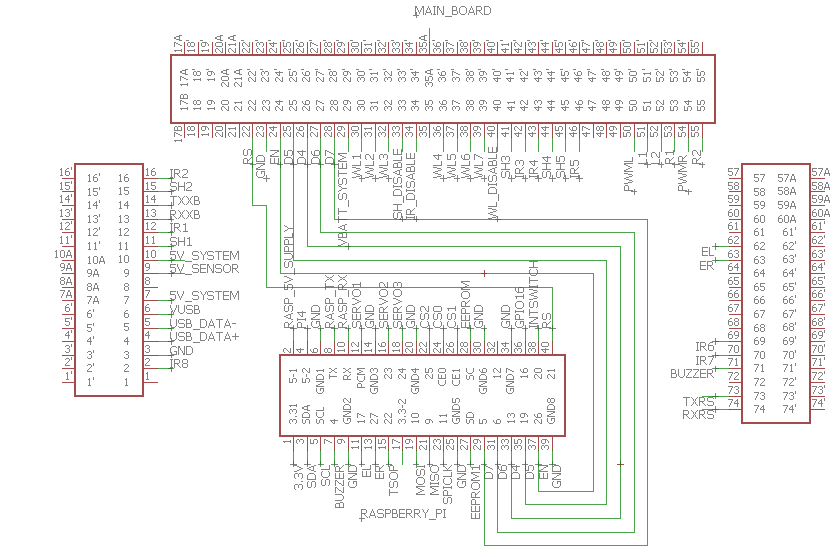
\includegraphics[width=1\textwidth]{lcd}
\end{figure}
\hfill
\begin{itemize}
	\item {LCD pins RS, EN, DB5, DB4, DB6 and DB7 are available on pins 22, 24, 25, 26, 27 and 28 resp. on the mainboard.}
	\item {These are give to pins 26, GND, 19, 13, 6, 5 and 21 gpio pins of raspberry pi resp.}
	\item {In order to program the LCD, these pins should be used.}
\end{itemize}
\pagebreak

\section*{\textbf{\fontsize{25}{10}\selectfont{7.Sensors and ADC interface}}}
\begin{figure}[h]
	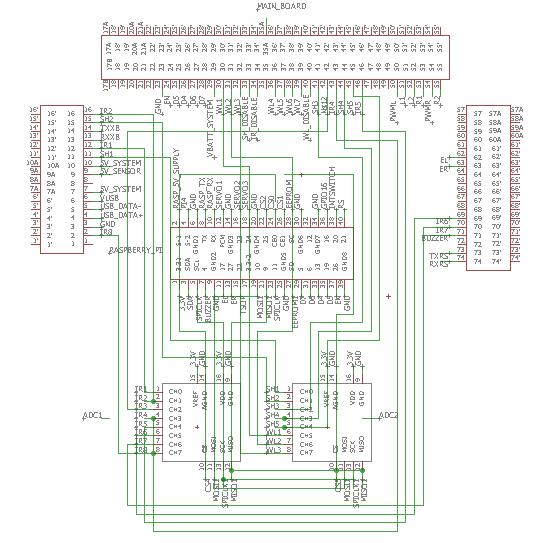
\includegraphics[width=1\textwidth]{adc}
\end{figure}
\hfill
\begin{itemize}
	\item {Sensors values are read by raspberry pi via external ADC. Raspberry pi communicates to ADC MCP3008 with SPI communication protocol.}
	\item {The communication between raspberry pi and MCP3008 happens with 3 lines, which are MISO, MOSI and SCLK. The appropriate device is chosen by its chip select pin which is unique for every device.}
	\item {All the 8 IR proximity sensors are connected to ADC1, White line sensors and sharp IR sensors are given to ADC2.}
\end{itemize}
\pagebreak

\section*{\textbf{\fontsize{25}{10}\selectfont{8.Motors and wheel encoders interface}}}
\begin{figure}[h]
	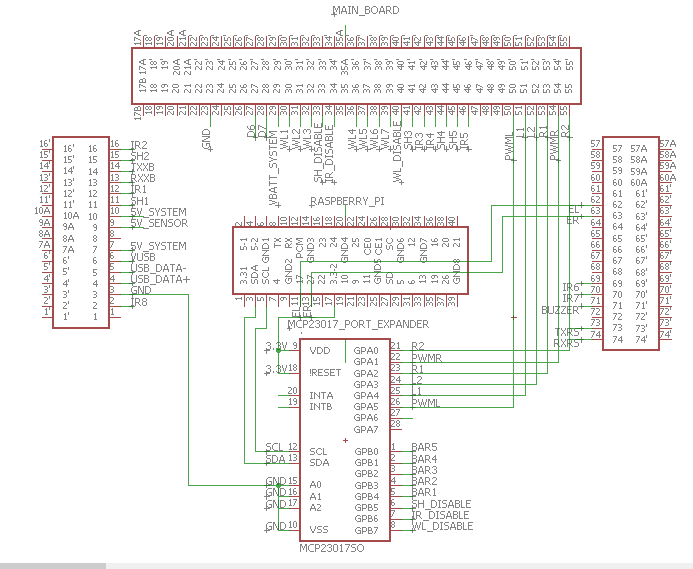
\includegraphics[width=1\textwidth]{wheels}
\end{figure}
\hfill
\begin{itemize}
	\item {Left motor control pins(L1,L2), Right motor control pins(R1,R2)and PWM motor control pins(PWMl, PWMR) are available on pins 51, 52, 53, 55, 50 and 54 pins of main board resp.}
	\item {The above mentioned pins are connected to MCP23017 Port expander with I2C communication.This would facilitate the usage of more GPIO pins since raspberry pi does'nt have many.}
	\item {Data and clk signals flow through SDA and SCL lines resp between Raspberry pi and MCP23017 port expander.}
	\item {The address of this Port expander as shown in fig. is 000 and that of 2nd is 001 which is specified by voltage levels at A0, A1, A2 pins resp.}
	\item {R2, PWMR, R1, L2, L1 and PWML pins are available on GPA0, GPA1, GPA2, GPA3, GPA4, GPA5 and GPA6 resp. of the Port expander.}
   	\item {The Left and Right wheel encoders are connected to the GPIO 17 and 27 pins of raspberry pi.}
\end{itemize}
\pagebreak

\section*{\textbf{\fontsize{25}{10}\selectfont{9.Powering servo motors and Servo pod connections}}}
\begin{figure}[h]
	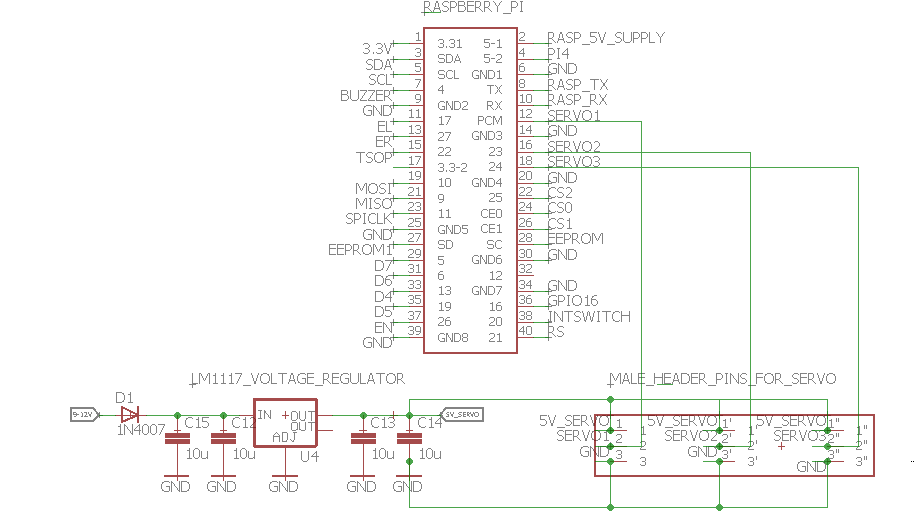
\includegraphics[width=1\textwidth]{servo}
\end{figure}
\hfill
\begin{itemize}
	\item {Servo motors need 5V and more than 500mA current to run efficiently. In order to meet these requirements, the +ve of servo motors is given to the output of LM1117 Voltage regulator IC. The input to which is given by 9-12V (pin 29) from main board.}
	\item {A set of 9 male header pins are given on the Adaptor board for interfacing upto 3 servo motors.}
	\item {Three of which are for Vcc (5V), three for ground and three for controlling th motion of servo motors 1,2 and 3 resp.}
	\item {The servo motor control pins are given to GPIO 5, 23 and 24 pins of raspberry pi resp. }
\end{itemize}
\pagebreak

\section*{\textbf{\fontsize{20}{10}\selectfont{10.Interrupt switch and controlling bargraph leds}}}
\begin{figure}[h]
	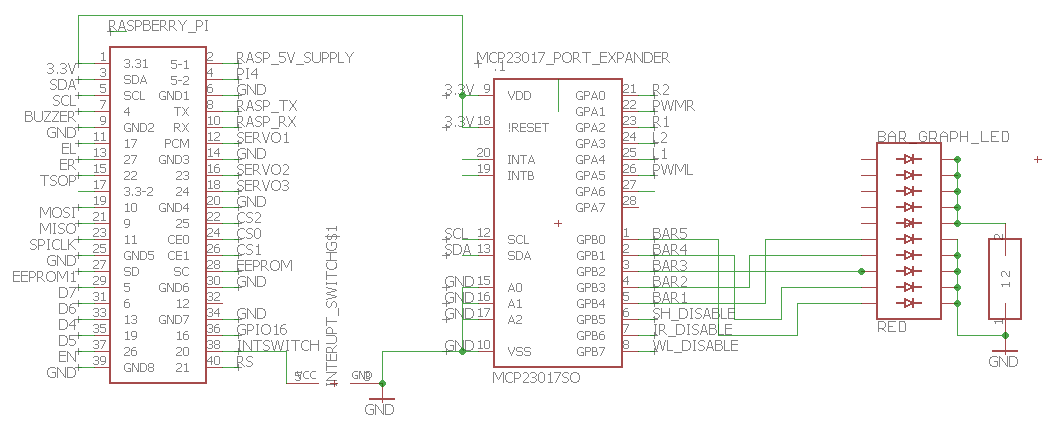
\includegraphics[width=1\textwidth]{interupt_bargraph}
\end{figure}
\hfill
\begin{itemize}
	\item {Sudden power cut to raspberry pi may lead to spoiling of the Raspbian OS. Hence, whenever the interrupt switch is pressed on the adaptor board, a python script could be written such that the raspberry pi shuts down systematically.}
	\item {The bottom 5 LEDs of bargraph LED can be controlled by the GPB0,  GPB1, GPB2, GPB3 and GPB4 pins of MCP23017 port Expander.}
\end{itemize}
\pagebreak

\section*{\textbf{\fontsize{20}{10}\selectfont{11.TSOP1738 RC5 IR receiver and decoder}}}
\begin{figure}[h]
	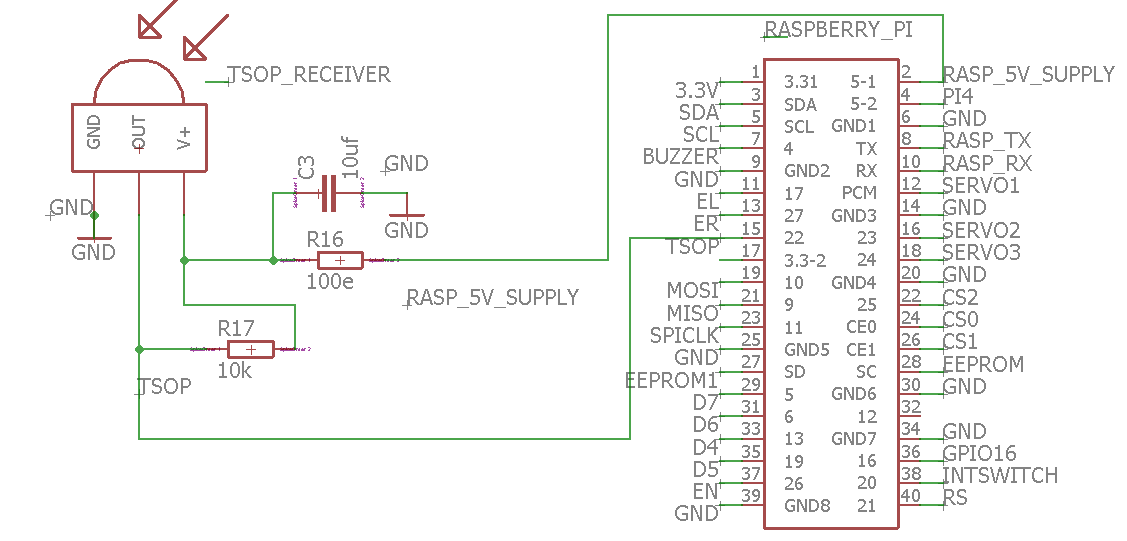
\includegraphics[width=1\textwidth]{tsop}
\end{figure}
\hfill
\begin{itemize}
	\item {The Firebird V robot can run according to the commands of TV remote, by decoding the IR signals which it receives from the TSOP receiver. }
	\item {It has Vcc(3.3V), ground and the output pin, which is connected to GPIO 22 pin rsapberry pi.}
	\item {By decoding the data obtained from the IR signals of TV remote, the robot could run accordingly.}
\end{itemize}
\pagebreak




\end{document}